\documentclass[nofootinbib,reprint,english]{revtex4-1}

% language
\usepackage[utf8]{inputenc}
\usepackage[english]{babel}

% standard setup
\usepackage{physics,amssymb,array}
\usepackage{xcolor,graphicx,hyperref}
\usepackage{tikz,listings,multirow}
\usepackage{algpseudocode,algorithm}
\usepackage{subcaption}
\usepackage{enumitem}

% hyperref coloring
\hypersetup{ %
  colorlinks,
  linkcolor={red!50!black},
  citecolor={blue!50!black},
  urlcolor={blue!80!black}}

% lstlisting coloring
\lstset{ %
  inputpath=,
  backgroundcolor=\color{white!88!black},
  basicstyle={\ttfamily\scriptsize},
  commentstyle=\color{magenta},
  language=Python,
  tabsize=2,
  numbers=left,
  stringstyle=\color{green!55!black},
  frame=single,
  keywordstyle=\color{blue},
  showstringspaces=false,
  columns=fullflexible,
  keepspaces=true}

\newcommand{\Y}{\vb{Y}}
\newcommand{\X}{\vb{X}}
\newcommand{\W}{\vb{W}}
\newcommand{\betahat}{\hat{\beta}}
\newcommand{\Eps}{\boldsymbol{\varepsilon}}
\newcommand{\yhat}{\hat{y}}
\newcommand{\phat}{\hat{p}}
\newcommand{\deltahat}{\hat{\delta}}

% no "do"'s
\algdef{SE}[FOR]{NoDoFor}{EndFor}[1]{\algorithmicfor\ #1}{\algorithmicend\ \algorithmicfor}
\algdef{SE}[FORALL]{NoDoForAll}{EndFor}[1]{\algorithmicfor\ #1}{\algorithmicend\ \algorithmicfor}
\algdef{SE}[IF]{NoThenIf}{EndIf}[1]{\algorithmicif\ #1}{\algorithmicend\ \algorithmicif}

\begin{document}
% titlepage
\title{FYS3155 Machine Learning - Project 2\\Supervised Machine Learning \& The Ising Model}
\author{Nils Johannes Mikkelsen}
\date{\today}
\noaffiliation
\begin{abstract}
Four supervised machine learning techinques are reviwed: linear regression, logistic regression, and MLP neural networks for regression and classification. The techniques are compared by analysing their performance with respect to the Ising model in one and two dimensions. The Lasso (linear regresion) method with a regularization strength of \(10^{-2}\) was particularly effective for the one-dimensional regression problem, the regression neural network performed poorly in comparison. The logistic regression was able to accurately label about 64\% of critical phase spin configrations. Meanwhile, a classification neural net was able to accurately predict 96.5\% of the critical states.
\end{abstract}
\maketitle

All material for project 2 may be found at:\\
{\scriptsize\url{https://github.com/njmikkelsen/machinelearning2018/tree/master/Project2}}

The original project description was accessed via the following link: \cite{project}\\
{\scriptsize\url{https://compphysics.github.io/MachineLearning/doc/Projects/2018/Project2/pdf/Project2.pdf}}

% body
\section{Introduction}
One of the most important set of tools available to a scientist is the wide range of statistical analysis techniques. Among the most famous of such techniques is the linear regression methods, whose range of applications span everything from aeronautical engineering to predictions of economic stability and the stock market. These methods date back over 200 years to the likes of Legendre (1805) and Gauss (1809), however, more recently more advanced techniques such artificial neural networks has proven itself much more useful in some areas. All of these methods are united under the umbrella term ``supervised machine learning'', it is the objective of this project to compare some of these supervised machine learning methods by studying the Ising model of ferromagnetism. In particular, this project will study the one-dimensional Ising model using linear regression and neural networks, and the two-dimensional Ising model using logistic regression and also neural networks. The focus of this report will not lie on the Ising model per sé, rather the performance of the supervised machine learning methods.
\section{Theory}
Most of the mathematics presented in this theory section is gathered from Trevor Hastie et al.'s \emph{The Elements of Statistical Learning} \cite{book}. Additional conventions and definitions are also inspired by Morten Hjorth-Jensen's lecture notes for FYS-STK 3155 \cite{notes}. Lastly, various code snippets in the project's code are partially inspired by Mehta et al.'s online notebooks \cite{notebooks}.
\subsection{The Ising Model}
The Ising model, named after \(20^\text{th}\) century German physicist Ernst Ising, is a mathematical description used to explain ferromagnetism as a macroscopic result of spin-spin interactions using statistical mechanics. The model arranges the atoms/molecules of a material, usually a metal, in a square \(n\)-dimensional lattice, each with a net spin of either +1 or -1. The mathematical description actually assumes an infinite-sized lattice, but this is usually mimicked via period boundary conditions. Furthermore, the model also assumes that an interaction between two spins \(s_i\) and \(s_j\) may only occur for neighbouring atoms/molecules and with a coupling strength of \(J\). Assuming no other interactions take place, the resulting Hamiltonian of the complete system is equal to
\begin{equation}
H=-J\sum_{\left\langle i,j\right\rangle}s_is_j
\end{equation}
where \(\left\langle i,j\right\rangle\) denotes a summation over all neighbouring spins. Seeing that systems of lower energy are more stable: if \(J>0\), then it is energetically favourable for the system to have aligned spins (such that \(s_is_j=1>0\)).

The one-dimensional case has been shown (analytically) not to experience a magnetic phase transition. For higher-dimensional cases however, the system does experience a phase transition.
\subsection{Supervised Machine Learning}
Regardless of their nature, all problems in statistical analysis may be decomposed into three components: some input data \(X\), some corresponding output data \(Y\) and a mathematical model \(f(X)\). Supervised machine learning (SML) is often used as an umbrella term for all statistical frameworks in which the output \(Y\) is known beforehand.

Furthermore, there are two major categories in SML: regression and classification. Both categories attempt to extract the underlying structure in the data (i.e., the statistical distribution that governs the data), however they differ in that while regression analysis attempts to estimate a quantity from the data, classification analysis attempts to place a label on the data. Mathematically speaking, regression models map the input (continuous or discrete) to a continuous output, while classification models map the input to a discrete output.

One of the difficulties in SML is to determine the mathematical model \(f\). The basis for all methods discussed in this project is the assumption that \(f\) maps the input \(X\) to \(Y\) with an error \(\varepsilon\):
\begin{equation}\label{eq:fundamental_assumption}
Y=f(X)+\varepsilon
\end{equation}
Different techniques place different assumptions on the statistical distribution of \(\varepsilon\).

The mathematical models are often parametrised such that one effectively imposes a \emph{class of models} as opposed to a single model. A common example would be an \(n^\text{th}\) degree polynomial approximation of some univariate data set \(\{(x_0,y_0),\ldots,(x_N,y_N)\}\), where the coefficients of the polynomial serve as the model's parameters. This leads to the fundamental mechanics of SML: determining the \emph{best} model in a class of models. This criteria of ``best'' arises naturally in the form of the \emph{cost function}, also known as the \emph{loss function}, which is an error function of \(f(X)\) with respect to \(Y)\). Depending on the choice of cost function, the resulting solution may be found using different methods.
\subsubsection{Regression}
It is not uncommon to know regression analysis as the concept of "function fitting", or in some cases simply "statistical modelling". While the latter term is unfitting in context of SML,\footnote{Pun intended.} the former term is more or less the core principle of regression analysis: to find the underlying functional form of the data set at hand. Consider figure \ref{fig:regression_example} in which the \(x\)-axis represent a one-dimensional input and the \(y\)-axis represents the one-dimensional output. It is tempting to speculate that the data would follow a linear curve exactly, had it been perfect.\footnote{By ``perfect'' it is implied that no error was made during the measurement process of the data.} This leads to the introduction of a linear model of the data; i.e. \(f(x)\) in figure \ref{fig:regression_example}. It is the problem of regression analysis to determine which linear curve, seeing that the data would not fit \emph{any} linear curve, would "fit the data the most" by minimising the cost function with respect the model class "linear curves". The general case is completely analogous: having chosen a class of models, regression analysis attempts to determine which specific model in the class that would minimise the chosen cost function.
\begin{figure}
\centering
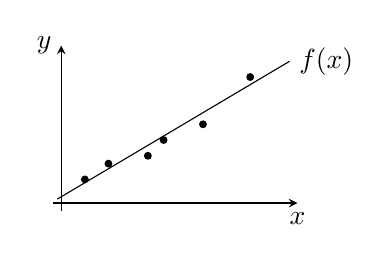
\begin{tikzpicture}
%axes
\draw[->,>=stealth] (-0.1,0) -- (3,0) node [pos=1.0,below] {\(x\)};
\draw[->,>=stealth] (0,-0.1) -- (0,2) node [pos=1.0,left]  {\(y\)};
%points
\fill[black] (0.3,0.3) circle [radius=0.05];
\fill[black] (0.6,0.5) circle [radius=0.05];
\fill[black] (1.1,0.6) circle [radius=0.05];
\fill[black] (1.3,0.8) circle [radius=0.05];
\fill[black] (1.8,1.0) circle [radius=0.05];
\fill[black] (2.4,1.6) circle [radius=0.05];
% line
\draw (-0.05,0.05) -- (2.9,1.8) node [pos=1.0,right] {\(f(x)\)};
\end{tikzpicture}
\caption{A simple example illustrating the general idea behind regression analysis: to extract the underlying functional form of data in the form of a continous function \(f\).}\label{fig:regression_example}
\end{figure}

\subsubsection{Classification}
Much like the name implies, classification analysis deals with the classifying, or labelling, of data. Consider for example trying to divide all cars into two categories: fast and slow cars. Now, one could impose an "acceleration" model that divides the cars based on how quickly a car reaches 100 km/h. In this case, it would be the problem of classification analysis to determine the time-interval after which a car must reach 100 km/h in order to be labelled "fast" as opposed to "slow". This is a binary model, however classification analysis is perfectly capable of handling models of greater dimensionality.
\subsection{Linear Regression}
The most common approach to regression analysis is known as ``Linear Regression''. Linear regression assumes that the output \(Y\) may be written as a linear combination of \(N\) models \(f_j(X)\), \(j\in\{1,\ldots,N\}\):
\begin{equation}\label{eq:linear_regression_fundamental_model}
Y=\beta_0+X_1\beta_1+\cdots+X_N\beta_N+\varepsilon=\beta_0+\tilde{Y}+\varepsilon
\end{equation}
where \(\beta_j\) are the coefficients of the expansion of \(Y\) in the basis \(\{f_j\}_{j=1}^N\). The coefficient \(\beta_0\) is known as the intercept, and is essentially a tool to center the output about 0. The object of linear regression is to determine the coefficients such that the cost function \(C(\beta)\) is minimised.

It is often the case that the set of inputs is large both in dimensionality \(N\) and in number of samples \(M\), providing equation \eqref{eq:linear_regression_fundamental_model} with an additional subscript \(i\in\{1,\ldots,M\}\): \(Y_i\), \(X_{ij}\), \(\beta_j\) and \(\varepsilon_j\) (where \(j\) is the initial subscript).  Hence it is effective to introduce a matrix-vector notation for \(Y\), \(X\) and \(\beta\). Let \(\Y\) be a \(M\)-dimensional column vector with entries \(Y_i-\beta_0\) and \(\betahat\) be a \(N\)-dimensional column vector with initial entry 1 and other entries \(\beta_j\). The inputs \(X_{ij}\) are combined into what is known as the design matrix:
\begin{equation}
\X=\mqty[
X_{11}  & \cdots & X_{1,N} \\
X_{21}  & \cdots & X_{2,N} \\
\vdots  & \ddots & \vdots  \\
X_{M,1} & \cdots & X_{M,N} ]
\end{equation}
In addition, the design matrix is often ``standardised'' by removing the mean from each column and dividing through by their standard deviations. With the final addition of the \(M\)-dimensional column vector \(\Eps\) (with entries \(\varepsilon_j\)), equation \eqref{eq:linear_regression_fundamental_model} may be rewritten as a matrix equation:
\begin{equation}\label{eq:linear_regression_matrix_equation}
\Y=\X\betahat+\Eps=\tilde{\Y}+\Eps
\end{equation}
where the \(j^\text{th}\) entry of \(\Y\), \(\X\betahat\) and \(\Eps\) constitute equation \eqref{eq:linear_regression_fundamental_model} for the \(j^\text{th}\) sample.

The next couple of subsections will first review three variants of linear regression before ending with an algorithm for estimating the final model's errors.
\subsubsection{Ordinary Least Squares}
In case of Ordinary Least Squares (OLS) the cost function is the Mean Squared Error (MSE):
\begin{subequations}\label{eq:MSE}
\begin{align}
\text{MSE}(\betahat)&=\frac{1}{M}\sum_{i=1}^M\big(Y_j-\tilde{Y}_j\big)^2\\
&=\big(\Y-\X\betahat\big)^T\big(\Y-\X\betahat\big)
\end{align}
\end{subequations}
The derivatives of MSE with respect to \(\betahat\) and \(\betahat^T\) are
\begin{subequations}
\begin{align}
\pdv{\text{MSE}(\betahat)}{\betahat}&=-2\X^T\big(\Y-\X\betahat\big)\label{eq:MSE_first_derivative}\\
\pdv{\text{MSE}(\betahat)}{\betahat^T}{\betahat}&=2\X^T\X\label{eq:MSE_second_derivative}
\end{align}
\end{subequations}
As the second derivative is strictly positive, the only minimum is the global minimum. Hence, the minimum is given by setting \eqref{eq:MSE_first_derivative} to zero:
\[-2\X^T\big(\Y-\X\betahat\big)=0\implies\X^T\Y=\X^T\X\betahat\]
such that
\begin{equation}\label{eq:OLS_solution}
\betahat=\big(\X^T\X\big)^{-1}\X^T\Y
\end{equation}
To compute \(\betahat\) using \eqref{eq:OLS_solution} is dependent on \(\X^T\X\) not being singular. This problem may be avoided via a Singular Value Decomposition (SVD):
\begin{equation}\label{eq:SingularValueDecomposition}
\X=\vb{U}\vb{D}\vb{V}^T
\end{equation}
where \(\vb{U}\) and \(\vb{V}\) are unitary matrices and \(\vb{D}\) is a diagonal matrix whose entries are the singular values of \(\X\). Using \eqref{eq:SingularValueDecomposition} on \eqref{eq:OLS_solution} yields

\begin{align*}
\betahat&=\Big[\big(\vb{U}\vb{D}\vb{V}^T\big)^T\big(\vb{U}\vb{D}\vb{V}^T\big)\Big]^{-1}\big(\vb{U}\vb{D}\vb{V}^T\big)^T\Y\\
&=\Big[\vb{V}\vb{D}^2\vb{V}^T\Big]^{-1}\vb{V}\vb{D}\vb{U}^T\Y\\
&=\vb{V}\vb{D}^{-2}\vb{V}^T\vb{V}\vb{D}\vb{U}^T\Y
\end{align*}
\begin{equation}\label{eq:OLS_solution_SVD}
\betahat=\vb{V}\vb{D}^{-1}\vb{U}^T\Y
\end{equation}
\subsubsection{Ridge Regression}
The origin of Ridge regression actually stems from problems with \(\X^T\X\) being singular. In order to approximate the solution, a small constant was added to diagonal of \(\X^T\X\). It was not until later that Ridge regression was formally explored and properly explained as linear regression with a cost function of
\begin{equation}\label{eq:Ridge_cost}
C_\text{Ridge}(\betahat;\lambda)=\text{MSE}(\betahat)+\lambda||\betahat||_2^2
\end{equation}
where the second term is known as a ``penalty''. Hence, Ridge regression is essentially OLS regression with an \(L^2\) penalty of the \(\beta\) coefficients that is parametrised by a so-called regularization parameter \(\lambda\). Note that the \(L^2\) penalty may be written as \(||\betahat||_2^T=\betahat^T\betahat\). The derivatives of the penalty term with respect to \(\betahat\) and \(\betahat^T\) are:
\begin{subequations}
\begin{align}
\pdv{L^2(\betahat)}{\betahat}&=2\lambda\betahat\label{eq:L2_first_derivative}\\
\pdv{L^2(\betahat)}{\betahat^T}{\betahat}&=2\lambda\label{eq:L2_second_derivative}
\end{align}
\end{subequations}
As \eqref{eq:L2_second_derivative} is positive, the second derivative of \(C_\text{Ridge}\) is also positive, thus the global minimum is also the only minimum in Ridge regression. Setting the first derivative of the cost function to zero one finds:
\[-2\X^T\big(\Y-\X\betahat\big)+2\lambda\betahat=0\implies \big(\X^T\X+\lambda\vb{I}\big)\beta=\X^T\Y\]
such that
\begin{equation}\label{eq:Ridge_solution}
\betahat_\text{Ridge}=\big(\X^T\X+\lambda\vb{I}\big)^{-1}\X^T\Y
\end{equation}
Again using the SVD (equation \eqref{eq:SingularValueDecomposition}) on \(\X\) one may avoid computation problems:
\begin{align*}
\betahat_\text{Ridge}&=\Big[\big(\vb{U}\vb{D}\vb{V}^T\big)^T\big(\vb{U}\vb{D}\vb{V}^T\big)+\lambda\vb{I}\Big]^{-1}\big(\vb{U}\vb{D}\vb{V}^T\big)^T\Y\\
&=\Big[\vb{V}\vb{D}^2\vb{V}^T+\lambda\vb{V}\vb{V}^T\Big]^{-1}\vb{V}\vb{D}\vb{U}^T\vb{Y}\\
&=\Big[\vb{V}\big(\vb{D}^2+\lambda\vb{I}\big)\vb{V}^T\Big]^{-1}\vb{V}\vb{D}\vb{U}^T\vb{Y}\\
&=\vb{V}\big(\vb{D}^2+\lambda\vb{I}\big)^{-1}\vb{V}^T\vb{V}\vb{D}\vb{U}^T\vb{Y}
\end{align*}
\begin{equation}\label{eq:Ridge_solution_SVD}
\betahat_\text{Ridge}=\vb{V}\big(\vb{D}^2+\lambda\vb{I}\big)^{-1}\vb{D}\vb{U}^T\vb{Y}
\end{equation}
\subsubsection{Lasso Regression}
Much like Ridge regression, Lasso regression adds a penalty to the cost function. However, whereas Ridge regression adds an \(L^2\) penalty, Lasso regression adds an \(L^1\) penalty:
\begin{equation}
C_\text{Lasso}(\betahat,\lambda)=\text{MSE}(\betahat)+\lambda||\betahat||_1
\end{equation}
Unlike OLS and Ridge regression, there does not exist a closed form solution for Lasso regression. Numerically stable and inexpensive algorithms for computing the solution do exist, one such algorithm is the Least Angle Regression (LAR) algorithm with the Lasso modification. However, as this project will implement \texttt{scikit-learn}'s \texttt{Lasso()} linear regressor class, the algorithms will not be further treated here.
\subsubsection{The Bias-Variance Decomposition}
Having analysed a regression problem using either OLS, Ridge or Lasso regression, the next step is to study the final model's prediction error. Consider the following expansion of the expected square error of the model:
\begin{align*}
\text{Err}(Y,\tilde{Y})&=\text{E}\Big[\big(Y-\tilde{Y}\big)^2\Big]=\text{E}\Big[Y^2-2Y\tilde{Y}+\tilde{Y}^2\Big]\\
&=\text{E}\big[Y^2\big]-2Y\text{E}\big[\tilde{Y}\big]+\text{E}\big[\tilde{Y}^2\big]
\end{align*}
where \(\text{E}\big[Y\big]=Y\). Assuming \(Y=\tilde{Y}+\varepsilon\), and placing the additional assumption that \(\text{E}\big[\varepsilon\big]=0\), it is clear that
\[\text{E}\big[Y\big]=\text{E}\big[\tilde{Y}+\varepsilon\big]=\text{E}\big[\tilde{Y}\big]=\tilde{Y}\]
Thus, the variance of \(Y\) is:
\[\text{Var}\big[Y\big]=\text{E}\Big[\big(Y-\text{E}\big[Y\big]\big)^2\Big]=\text{E}\Big[\big(\tilde{Y}+\varepsilon-\tilde{Y}\big)^2\Big]=\text{E}\big[\varepsilon^2\big]\]
To simplify notation, let \(\sigma_\varepsilon^2=\text{Var}\big[\varepsilon\big]\) such that
\[\sigma_\varepsilon^2=\text{E}\big[\varepsilon^2\big]-\text{E}\big[\varepsilon\big]^2=\text{E}\big[\varepsilon^2\big]-0=\text{Var}\big[Y\big]\]
as \(\text{E}\big[\varepsilon\big]=0\). The error can therefore be rewritten as
\begin{align*}
\text{Err}(Y,\tilde{Y})&=\text{Var}\big[Y\big]+\text{E}\big[Y\big]^2-2Y\text{E}\big[\tilde{Y}\big]\\
&\quad+\text{Var}\big[\tilde{Y}\big]+\text{E}\big[\tilde{Y}\big]^2\\
&=\sigma_\varepsilon^2+\text{Var}\big[\tilde{Y}\big]+Y^2-2Y\text{E}\big[\tilde{Y}\big]+\text{E}\big[\tilde{Y}\big]^2\\
&=\sigma_\varepsilon^2+\text{Var}\big[\tilde{Y}\big]+\Big(Y-\text{E}\big[\tilde{Y}\big]\Big)^2
\end{align*}
or in other words:
\begin{equation}\label{eq:bias_variance_decomposition}
\text{Err}(Y,\tilde{Y})=\sigma_\varepsilon^2+\text{Var}\big[\tilde{Y}\big]+\text{Bias}\big[Y,\tilde{Y}\big]^2
\end{equation}
Equation \eqref{eq:bias_variance_decomposition} is known as the Bias-Variance decomposition of the squared error. The term \(\sigma_\varepsilon^2\) is known as the \emph{irreducible} error of the model, and is an error due to variance in the data set. On the other hand, \(\text{Var}\big[\tilde{Y}\big]\) and \(\text{Bias}\big[Y,\tilde{Y}\big]\) are known as the variance and bias of the model. In general, there are no closed form expressions for these quantities, but there are rigurous algorithms for approximating them. One such technique is the Bootstrap resampling technique, which is introduced in the next section.
\subsubsection{The Bootstrap Resampling Technique}
Having introduced different methods in linear regression, this section will review the Bootstrap resampling technique, which is a statistical tool for assessing a model's prediction error. The general idea is to estimate a given statistic using the average statistic over a number of resampled training sets. The Bootstrap will only be used in conjunction with linear regression in this project, but it is equally applicable in other fields such as logistic regression and neural networks.

There are many variants of Bootstrapping, this project will employ one of the standard ones. Provided a data set with inputs and outputs \(D=\{\vb{d}_0,\ldots,\vb{d}_N\}\), a ``Bootstrap sample'' \(B\) refers to a data set with \(N\) elements picked at random from \(D\) with replacement. The ``with replacement'' component is crucial as it ensures that an element in \(D\) may occur in \(B\) several times. Having chosen a statistic \(A(D)\), the Bootstrap estimate of the true value of \(A(D)\) is the average of \(A\) computed over several Bootstrap samples (here \(M\) samples):
\begin{equation}
A(D)\cong\frac{1}{M}\sum_{i=1}^M A(B_i)
\end{equation}
where \(B_i\) denotes the \(i^\text{th}\) Bootstrap data set drawn at random.

When it comes to the Bootstrap, this project is mostly interested in estimating a model's bias-variance decomposition. Say a model's output is \(\hat{\theta}\) and the model's target is \(\theta\), the Bootstrap estimates for the model Bias and Variance of \(\hat{\theta}\) are:
\begin{subequations}
\begin{align}
\text{Bias}(\theta,\hat{\theta})&=\frac{1}{M}\sum_{i=1}^M\big(\hat{\theta}_i-\theta\big)\\
\text{Var}(\theta,\hat{\theta})&=\frac{1}{MN}\sum_{i=1}^M\big(\hat{\theta}_i-\theta\big)^2
\end{align}
\end{subequations}
where \(\hat{\theta}_i\) is the model's ouput computed from the \(i^\text{th}\) Bootstrap sample.
\section{Logistic Regression}
Logistic regression, in contrast to its name, is one of the standard apporaches to classification analysis. A logistic regression model that contains \(K\) classes would assign each input a probability of residing in each of the \(K\) classes, then classify the input according to the largest probability. The ``regression'' in logistic regression actually arises from how the probabilities are modelled according to a regression model. The mechanics of logistic regression are based on the logistic function, or logit transformation:
\begin{equation}\label{eq:logit_transformation}
p(t)=\frac{1}{1+e^{-t}}=\frac{e^t}{1+e^t}
\end{equation}
which represents the likelihood of labelling an input with a specific class.

Because this project will only employ the binary logistic regression model, i.e. logistic regression with only 2 classes, the following section will simplify the mathematics to the binary case. One of the simplest binary output labelling systems is \(y_i\in\{0,1\}\). Using this labelling, the probabilities of classifying an input \(\vb{x}_i\) with output \(y_i=0\) or \(y_i=1\), provided model parameters \(\betahat\), may be written as:
\[p(y_i=0|\vb{x}_i,\betahat)=p_i\qand p(y_i=1|\vb{x}_i,\betahat)=1-p_i\]
The regression model of logistic regression may thus be expressed as
\begin{equation}
\ln\bigg(\frac{p_i}{1-p_i}\bigg)=\betahat^T\vb{x}_i
\end{equation}
Note that the \(t\) parameter passed to the logit transformation (equation \eqref{eq:logit_transformation}) in logistic regression is \(\betahat^T\vb{x}_i\). Furthermore, it is common practice to pad a 1 to the input vector and an intercept term \(\beta_0\) to the parameter vector in order to center the data.

Seeing that logistic regression \emph{is} a regression problem, there must be some cost function that determines the success of a model; for logistic regression this is the cross-entropy.\footnote{Actually, logistic regression is based on maximising the so-called maximum likelihood. However, this is equivalent with minimising the cross-entropy.} Provided an input matrix \(\X\) (with input vectors \(\vb{x}_i\) as rows) may be written as
\begin{equation}\label{eq:C_cross_entropy}
C_\times(\betahat)=-\sum_{i=1}^N\Big[y_i\betahat^T\X-\ln\big(1+e^{\betahat^T\X}\big)\Big]
\end{equation}
Following the derivations of linear regression methods, the optimal parameters are found by analysing the derivative of \(C_\times\) with respect to \(\betahat\) and \(\betahat^T\):
\begin{subequations}\label{eq:C_cross_derivatives}
\begin{align}
\pdv{C_\times(\betahat)}{\betahat}&=-\X^T\big(\yhat-\phat\big)\label{eq:C_cross_first_derivative}\\
\pdv{C_\times(\betahat)}{\betahat^T\betahat}&=\X^T\W\X\label{eq:C_cross_second_derivative}
\end{align}
\end{subequations}
where \(\yhat\) and \(\phat\) are column vectors with entries \(y_i\) and \(p_i\) and \(\W\) is a weight matrix with entries \(p_i(1-p_i)\).

Unlike linear regression, \eqref{eq:C_cross_second_derivative} is not necessarily strictly positive. Thus, the global minimum is not necessarily the only minimum. The minimum is found where \eqref{eq:C_cross_first_derivative} is equal to zero, but there is no closed form expression for the corresponding parameter vector \(\betahat_\times\). Thus, the solution is found via iterative schemes such as gradient descent, Newton-Raphson's method, etc. This project employs gradient descent both with logistic regression and with neural networks, which is why a discussion of gradient descent is postponed until after neural networks have been introduced.

Like linear regression, the cost function is often given an additional \(L^1\) or \(L^2\) penalty (or a mixture of the two). From the discussion in the linear regression section, it is clear that such a penalty would not affect the global minmium in any significant way. Thus, the solution would still need to be found via iterative schemes.
\section{Gradient Descent Methods}
Gradient descent methods is an umbrella term for iterative optimalisation methods for multivariate scalar fields \(\phi(\vb{x})\). The aim of these methods is to find the minimum of \(\phi\), assuming it exists. There are countless variations of the gradient descent, but the standard formulation is:
\begin{equation}\label{eq:standard_gradient_descent}
\vb{x}_{n+1}=\vb{x}_n-\eta_n\nabla\phi(\vb{x}_n)
\end{equation}
The simplest version of \eqref{eq:standard_gradient_descent} is found when the step length \(\eta_n\) is chosen to be constant and the procedure is continued for a given number of steps, say \(N\). In this case, convergence is neither guaranteed nor very likely. Another difficulty with gradient descent methods is their strong sensitivity to initial conditions. In case the simple gradient descent has difficulty in finding the minmium, it is often reasonble to perform a grid search of initial conditions in order to reduce the potential of an unfortunate \(\vb{x}_0\).

One way to improve the likelihood of finding the global minimum of \(\phi\) is to introduce the stochastic gradient descent (SGD). This variant of gradient descent arises from the desire to optimise a scalar field with respect to some other input \(\vb{y}\). In this case, \(\vb{x}\) is consider a parameter-vector, while \(\vb{y}\) is considered the actual input of \(\phi\). That is, the aim of SGD is to optimise \(\phi(\vb{y};\vb{x})\) in terms of \(\vb{x}\), where \(\vb{y}\in\{\vb{y}_1,\ldots,\vb{y}_M\}\) is considered constant. What SGD does is to use the average gradient from a random sample. The set of \(\vb{y}\) inputs is divided into \(K\) so-called batches \(B_k\), which are subsets of \(\{\vb{y}_1,\ldots,\vb{y}_M\}\) with \(M/K\) elements. The equivalent gradient in SGD to \eqref{eq:standard_gradient_descent} is then
\begin{equation}\label{eq:batch_average_gradient}
\nabla_ {\vb{x}}\phi(\vb{y};\vb{x})=\sum_{k\in B_k}^K\nabla_{\vb{x}}\phi(\vb{y}_k,\vb{x})
\end{equation}

Moving on, an additional improvement to batch training is to use a varying learning rate \(\eta_n\). A natural choice would be to adjust \(\eta_n\) with each iteration, but this often leads to the minimum not being achieved. To circumvent this, a common strategy is to learn in so-called ``epochs''. In this terminology, one epoch refers to one iteration across every batch in the set of batches. It is also common to improve this further by introducing combining this epochs-approach with SGD, such that instead of iterating over every batch, one epoch includes an iteration over \(K\) (the number of batches) batches drawn at random with replacement. There is no best way of updating the learning rate, the only criteria is \(0<\eta_{n+1}<\eta_n\). A common way is to use an exponential falloff:
\begin{equation}\label{eq:exp_falloff_learning_rate}
\eta_n=\eta_0 e^{-n\alpha}
\end{equation}
where \(\eta_0\) is the initial learning rate, \(n\) is the number of completed epochs and \(0<\alpha\) is a falloff parameter. Alternatively, equation \eqref{eq:exp_falloff_learning_rate} may be written as
\begin{equation}
\eta_{n+1}=\eta_n e^{-\alpha}\qq{provided}\eta_0
\end{equation}
\section{The Multi-Layered Perceptron}
The final SML tool used in this project is the Multi-Layered Perceptron (MLP) Neural Network, which is essentially a multi-stage regression and or classification model with non-linear stage-to-stage mapping. That is, an MLP network is composed of several stages, called layers, that manipulate the data in two ways: through a regression/classification transformation, and through a non-linear map. Unlike more advanced networks, an MLP is restricted to a linear structure of the layers, meaning the input data is sent through each layer one-by-one. There are three kinds of layers: the input layer, the output layer and hidden layers. The input and output layers are trivial, their only criteria is that of a linear map such that the network's output is not restricted. A hidden layer is any layer inbetween the input and output layers. Hidden layers are  the essential components of an MLP, because their action is strictly non-linear.
\subsubsection{The fundamentals of MLPs}
A hidden layer is comprised of several ``nodes'' that are the gateways through which data is passed. The connections between nodes are the possible paths of the input data, thus their structure is very important. In the case of MLPs, each node is isolated from every other node in the same layer, but is connected to every node in the previous and next layers. The idea is illustrated in figure \ref{fig:node_connections}: Each connection is given a weighting \(w_{ij}\) that determines the amount of the signal from the \(j^\text{th}\) node in the previous layer, that will contribute to the \(i^\text{th}\) node in the current layer. In addition to the weighted output from the previous layer, a bias \(b_i\) is also supplied to current layer. This bias functions as the intercept in regression analysis. The input received by node \(i\) can be expressed as:
\begin{equation}
z_i=\sum_{j=1}^{N_\text{prev}}w_{ij}x_j+b_i
\end{equation}
where \(N_\text{prev}\) is the number of nodes in the previous layer.

\begin{figure}
\centering
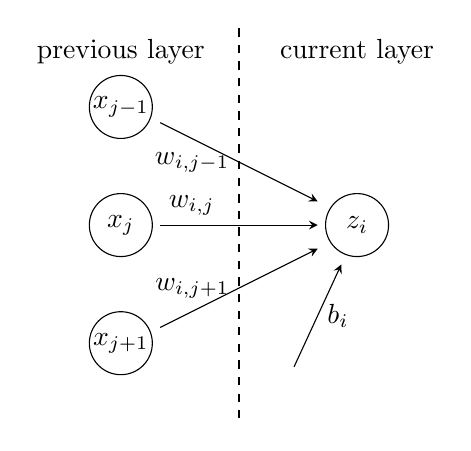
\begin{tikzpicture}
\draw (1,0) circle [radius=0.4];
\draw node at (1,0) {\(z_i\)};

\draw (-2,+1.5) circle [radius=0.4];
\draw (-2,+0.0) circle [radius=0.4];
\draw (-2,-1.5) circle [radius=0.4];

\draw node at (-2,+1.5) {\(x_{j-1}\)};
\draw node at (-2,+0.0) {\(x_{j}\)};
\draw node at (-2,-1.5) {\(x_{j+1}\)};

\draw[->,>=stealth] (-2,+1.5) + (0.5,-0.2) -- (0.5,+0.3) node [pos=0.5,left] {\(w_{i,j-1}\)};
\draw[->,>=stealth] (-2,+0.0) + (0.5,+0.0) -- (0.5,+0.0) node [pos=0.2,above] {\(w_{i,j}\)};
\draw[->,>=stealth] (-2,-1.5) + (0.5,+0.2) -- (0.5,-0.3) node [pos=0.5,left]  {\(w_{i,j+1}\)};

\draw[->,>=stealth] (0.2,-1.8) -- (0.8,-0.5) node [pos=0.5,right] {\(b_i\)};

\draw node at (+1,2.2) {current layer};
\draw node at (-2,2.2) {previous layer};

\draw[dashed] (-0.5,2.5) -- (-0.5,-2.5);
\end{tikzpicture}
\caption{An illustration of how the nodes in hidden layers are interconnected. The input received by a node \(i\) in the current layer is composed of a bias \(b_i\) and a weighted signal from each of the nodes of the previous layer.}\label{fig:node_connections}
\end{figure}

Upon receiving the weighted input \(z_i\), the node undergoes a process known as activation. In short the node input \(z_i\) is passed through a non-linear map \(f_i\) known as the activation function. Common activation functions include the logistic function (equation \eqref{eq:logit_transformation}), \(\tanh(x)\), and several others. The output from the node is thus
\begin{equation}\label{eq:node_output}
y_i=f_i(z_i)=f_i\Bigg(\sum_{j=1}^{N_\text{prev}}w_{ij}x_j+b_i\Bigg)
\end{equation}
which is sent to the next layer, etc.

The mathematics of matrix notation may be elegantly exploited to extend \eqref{eq:node_output} to the general case. Let the previous and current layers be denoted as layers \(l-1\) and \(l\) respectively. The weights \(w_{ij}^l\) for the \(l^\text{th}\) layer are arranged in a weight matrix \(\W^l\) with dimensions \(N_l\times N_{l-1}\), meanwhile the input signals from each node in layer \(l-1\) (that is \(x_j\)) are arranged in the \(N_{l-1}\)-dimensional column vector \(\vb{y}^{l-1}\). The weighted inputs for layer \(l\) are then given by \(\W\vb{y}_{l-1}\) such that the outputs of layer \(l\) are given by:
\begin{equation}\label{eq:node_output_matrix}
\vb{y}^l=f_l(\vb{z}^l)=f_l\big(\W^l\vb{y}^{l-1}+\vb{b}^l\big)
\end{equation}
where \(\vb{b}^l\) is the \(N_l\)-dimensional column vector with biases \(b_i^l\). With a total number of \(L\) hidden layers, the network output may thus be written in terms of the network inputs as:
\begin{equation}\label{eq:equation_of_neural_network}
\vb{y}=f_L\bigg(\W^Lf_{L-1}\bigg(\cdots \bigg(\W^1\vb{x}+\vb{b}^1\bigg)\cdots\bigg)+\vb{b}^L\bigg)
\end{equation}
Equation \eqref{eq:equation_of_neural_network} is really important, because it shows what a neural network really is: it's ``just'' a plain mathematical map of the inputs \(\vb{x}\) to the  outputs \(\vb{y}\) with parameters \(\{(\W^1,\vb{b}^1),\ldots,(\W^L,\vb{b}^L)\}\). Different neural networks represent different mathematical maps, whose applicability depends on the problem at hand. Mirroring linear regression and logistic regression, the success of a neural network is measured via the cost function. The choice of cost function and the choice of network design varies greatly from data set to data set. 
\subsubsection{Fitting the MLP: The back-propagation algorithm}
Much like linear and logistic regression, fitting an MLP is a process of minimising the cost function \(C(\vb{y})\). For MLPs, the cost function is dependent on all weights and biases in the network. The basic idea behind the back-propagation algorithm is to update the network weights and biases via an iterative process using methods such as gradient descent. The algorithm is divided into two steps: a forward sweep (or ``feed forward'') and the so-called back-propagation.

The forward sweep is the easiest step. It involves computing the network output \(\vb{y}\) from the network input \(\vb{x}\) using \eqref{eq:equation_of_neural_network}. Computationally speaking, this is usually done by iterating over the network layers and compute the layer outputs one-by-one.

Once the forward sweep is completed, the next step is to update the weights and biases via back-propagation. The mathematics are essentially the same as for linear and logistic regression: the optimal weights and biases are determined such that the first derivative of the cost function is zero. Ideally one would find the derivative of the cost function with respect to every parameter, however, this can be greatly simplified using the symmetric nature of equation \eqref{eq:node_output_matrix}. The idea is to find the derivative of the cost function with respect to the weights and biases of the final layer (i.e. layer \(L\)), and then compute the derivatives with respect to weights and biases of earlier layers using a recursive strategy. This recursive computation scheme is the ``backwards propagation'' in the back-propagation algorithm.

Seeing that equation \eqref{eq:equation_of_neural_network} is continuous in all the weights and biases, the cost function \(C(\vb{y})\) may be studied with respect to the weights and biases of any layer, say layer \(l\). This implies that its derivatives with respect to the weights and biases of layer \(l\) are:
\begin{subequations}\label{eq:nerual_network_chain_derivatives}
\begin{align}
\pdv{C}{\W^l}&=\pdv{C}{\vb{y}^l}\ \pdv{\vb{y}^l}{\vb{z}^l}\ \pdv{\vb{z}^l}{\W^l}\\
\pdv{C}{\vb{b}^l}&=\pdv{C}{\vb{y}^l}\ \pdv{\vb{y}^l}{\vb{z}^l}\ \pdv{\vb{z}^l}{\vb{b}^l}
\end{align}
\end{subequations}

The first term in equations \eqref{eq:nerual_network_chain_derivatives}, i.e. \(\pdv*{C}{\vb{y}^l}\), is dependent on the choice of cost function \(C\). The two most common choices are the Squared Error and Cross-Entropy:
\begin{subequations}
\begin{align}
&\text{Squared Error:}\nonumber\\
&C(\vb{y},\vb{t})=\frac{1}{2}\big(\vb{y}-\vb{t}\big)^T\big(\vb{y}-\vb{t}\big) \\
&\text{Cross Entropy:}\nonumber\\
&C(\vb{y},\vb{t})=-\Big[\vb{t}^T\ln\big(\vb{y}\big)+\big(\vb{1}-\vb{t}\big)^T\ln\big(\vb{1}-\vb{y}\big)\Big]\label{eq:neural_networks_cross_entropy}
\end{align}
\end{subequations}
where \(\vb{t}\) are the targets, i.e. the desired network outputs. The derivative of these cost functions are
\begin{subequations}
\begin{align}
&\text{Squared Error:}\nonumber\\
&\pdv{C(\vb{y},\vb{t})}{\vb{y}}=\vb{y}-\vb{t} \\
&\text{Cross Entropy:}\nonumber\\
&\pdv{C(\vb{y},\vb{t})}{\vb{y}}=\big[\vb{y}-\vb{t}\big]\oslash\Big[\vb{y}\circ\big(\vb{1}-\vb{y}\big)\Big]
\end{align}
\end{subequations}
where \(\oslash\) and \(\circ\) denote Hadamard division and multiplication.

The second term in equations \eqref{eq:nerual_network_chain_derivatives}, i.e. \(\pdv*{\vb{y}^l}{\vb{z}^l}\), is dependent on the choice of activation function \(f_l\):
\begin{equation}\label{eq:derivative_activation}
\pdv{\vb{y}^l}{\vb{z}^l}=\pdv{\vb{z}^l}f_l\big(\vb{z}^l\big)=f_l'\big(\vb{z}^l\big)
\end{equation}
Common activation functions include (but are not limited to) the logistic function, the hyperbolic tangent, the identity function and the softmax function. The hyperbolic tangent and the identity function are trivial, the logistic function is listed in equation \eqref{eq:logit_transformation}, the only remaining function is the softmax function:
\begin{equation}\label{eq:softmax}
\text{softmax}(i,\vb{x})=\frac{e^{x_i}}{\sum_{n=1}^Ne^{x_n}}
\end{equation}
For computational reasons, the softmax is often evaluated using:
\[\text{softmax}(i,\vb{x})=\frac{e^{x_i-\max x}}{\sum_{n=1}^Ne^{x_n-\max x}}\]
in order to avoid overflow. The derivatives of the first three activation functions are simple:
\begin{subequations}\label{eq:activation_derivatives}
\begin{align}
\text{logit}'(x)&=\text{logit}(x)\big(1-\text{logit}(x)\big)\\
\tanh'(x)&=1-\tanh^2(x)\\
\text{identity}'(x)&=1\\
\intertext{The derivative of the softmax however is slightly more complicated, but only because it accepts a vector and an index as arguments. Its derivative is therefore index-dependent:}
\pdv{x_k}\text{softmax}(i,\vb{x})&=\text{softmax}(i,\vb{x})\nonumber\\
&\quad\cdot\big(\delta_{ik}-\text{softmax}(i,\vb{x})\big)
\end{align}
\end{subequations}
Note that all the derivatives in \eqref{eq:activation_derivatives} are given in terms of their corresponding function values. This is due to computational considerations: the function values are computed during the forward sweep. Several of these derivatives contain exponentials, which becomes computationally very expensive to evaluate for large number of iterations.

The final terms in equation \eqref{eq:nerual_network_chain_derivatives}, i.e. \(\pdv*{\vb{z}^l}{\vb{\W}^l}\) and \(\pdv*{\vb{z}^l}{\vb{b}^l}\), are actually the simplest:
\begin{equation}\label{eq:z_derivatives_W_and_b}
\pdv{\vb{z}^l}{\vb{\W}^l}=\big[\vb{y}^{l-1}\big]^T\qand\pdv{\vb{z}^l}{\vb{b}^l}=1
\end{equation}
which follows from \(\vb{z}^l=\W^l\vb{y}^{l-1}+\vb{b}^l\).

Having studied each component of equations \eqref{eq:nerual_network_chain_derivatives}, the next step is to introduce an essential quantity in neural networks, the so-called signal error:
\begin{equation}\label{eq:signal_error_definition}
\deltahat^l\equiv\pdv{C}{\vb{z}^l}=\pdv{C}{\vb{y}^l}\circ f'(\vb{z}^l)
\end{equation}
which appears in equations \eqref{eq:nerual_network_chain_derivatives} with \(\vb{y}^l=f(\vb{z}^l)\). The signal error is the quantity that is back-propagated during a back-propagation. This is because the signal error may be written as a recursive sequence by exploiting the chain rule:
\[\pdv{C}{\vb{y}^l}=\pdv{C}{\vb{z}^{l+1}}\ \pdv{\vb{z}^{l+1}}{\vb{y}^l}=\Big[\big[\deltahat^{l+1}\big]^T\W^{l+1}\Big]^T=\big(\W^{l+1}\big)^T\deltahat^{l+1}\]
where the awkward transpose-notation is for preserving the dimensions of \(\pdv*{C}{\vb{y}^l}\) (otherwise it would become a row vector instead of a column vector).

Having introduced the necessary theory and jargon, the equations of back-propagation are now ready to be presented (in all their glory):
\begin{subequations}\label{eq:back_propagation_equations}
\begin{align}
\deltahat^L&=\pdv{C}{\vb{y}^L}\circ f'(\vb{z}^L)\label{eq:initial_signal_error}\\
\deltahat^l&=\big(\W^{l+1}\big)^T\deltahat^{l+1}\circ f'(\vb{z}^l)\label{eq:recursive_signal_error}\\
\pdv{C}{\W^l}&=\deltahat^l\big[\vb{y}^{l-1}\big]^T\label{eq:nerual_network_weight_derivative}\\
\pdv{C}{\vb{b}^l}&=\deltahat^l\label{eq:neural_network_bias_derivative}
\end{align}
\end{subequations}
Here, equation \eqref{eq:initial_signal_error} is found by applying \eqref{eq:signal_error_definition} at \(l=L\), and equation \eqref{eq:recursive_signal_error} follows directly by inserting the chain rule expression into \eqref{eq:signal_error_definition}. Equations \eqref{eq:nerual_network_weight_derivative} and \eqref{eq:neural_network_bias_derivative} are found by inserting \eqref{eq:z_derivatives_W_and_b} and \eqref{eq:signal_error_definition} into equations \eqref{eq:nerual_network_chain_derivatives}.

With explicit expressions for the derivative of the cost function with respect to all weights and biases, gradient methods may be used to optimise the network. The final back-propagation algorithm is:
\begin{algorithm}[H]
\caption{Neural Network Back-Propagation}\label{alg:back_propagation}
\begin{algorithmic}[1]
\State Initialise network weights and biases.
\NoDoFor {\(i=1,\ldots,N\):}
	\State Feed input \(\vb{x}\) forward.
	\State Compute \(\deltahat^L\).
	\NoDoFor {\(l=L-1,\ldots,1\):}
		\State Compute \(\deltahat^l\).
	\EndFor
	\NoDoFor {\(l=1,\ldots,L-1\):}
		\State Update \(\W^l\) and \(\vb{b}^l\) via a gradient descent step.
	\EndFor
\EndFor
\end{algorithmic}
\end{algorithm}
Variants of the algorithm may involve training in batches instead of with a single input vector. Implementing this is easy as the mathematics are invariant of the row-dimensionality of \(\vb{x}\). This implies that Algorithm \ref{alg:back_propagation} and equations \eqref{eq:back_propagation_equations} would require no alteration if supplied an input matrix \(\X\) with input vectors \(\vb{x}_i\) as columns. The only meaningful difference in the mathematics is that the quantites \(\deltahat^l\), \(\vb{z}^l\) and \(\vb{y}^l\) would become matrices, the dimensionality of \(\W^l\) and \(\vb{b}^l\) would remain unchanged. To update \(\W^l\) and \(\vb{b}^l\), one would typically choose the average column of \(\deltahat^l\) as the signal-error.

\section{Method}
The main focus of this project is use the Ising model as a base for comparing the different SML  techniques/methods presented in the theory section. The project will restrict the model to the one-dimensional case and the two-dimensional case. The one-dimensional case will be analysed using a standard linear regression approach, and with a Squared-Error nerual network. The two-dimensional case will be analysed using logistic regression, and with a Cross-Entropy nerual network.
\subsection{Preparation}
Before proceding to the statistical methods, the first problem is to find access to Ising data sets. This will be done differently for the one-dimensional case and the two-dimensional case: Data sets for the one-dimensional case will be designed from scratch using simple \texttt{Python} code. On the other hand, data sets for the two-dimensional case will be downloaded from Mehta et al's online repository:\\
{\scriptsize\url{https://physics.bu.edu/~pankajm/ML-Review-Datasets/isingMC/}}\\

The following mathematics outline the equations needed for generating one-dimensional data sets: The one-dimensional Hamiltonian may be written as
\begin{equation}\label{eq:one_dim_Ising_Hamiltonian}
H^1(\vb{s})=-J\sum_{j=1}^Ns_js_{j+1}
\end{equation}
where \(s_j=\pm1\) is the \(j^\text{th}\) spin in a one-dimensional lattice, or chain, of spins:
\[\vb{s}=\mqty[s_1&s_2&\cdots&s_N]\]
Note that the final spin-coupling \(s_Ns_{N+1}\) is handled using period boundary conditions: \(s_{N+1}=s_1\). Using this notation, a single data set would be the set \(\{\vb{s},H^1(\vb{s})\}\). Now let \(\vb{s}^i\) denote the \(i^\text{th}\) random-generated chain of spins such that \(\{\vb{s}^i,H^1(\vb{s}^i)\}\) becomes the \(i^\text{th}\) data set. The following code exploits some clever \texttt{NumPy} functionality for generating \texttt{M} data sets of dimensionality \texttt{N} (number of spins per chain) with coupling constant \texttt{J}. The code is inspired by the code listed on this page:\\
{\scriptsize\url{https://physics.bu.edu/~pankajm/ML-Notebooks/HTML/NB_CVI-linreg_ising.html}}
\begin{lstlisting}[caption={\texttt{Python 3} code for generating 1D data sets},label={lst:generate_1D_data}]
# generate M N-dimensional chains of spins
states = np.random.choice([-1,1],size=(self.M,self.N))
states = np.asarray(states,dtype=np.int8)
# find non-zero contributions to Hamiltonian
E = np.zeros((self.N,self.N),)
for i in range(self.N):
	E[i,(i+1)%self.N] -= self.J
# compute Hamiltonian
H = np.einsum('...i,ij,...j->...',states,E,states)
\end{lstlisting}
With the data sets in hand, the next step is to rephrase the problem such that the statistical models may be used. The mathematics will be framed from the persepctive of the one-dimensional model, but the \(n\)-dimensional case is completely analogous.


In complete ignorance of the Ising model, it would be unreasonable to suggest that only neighbouring spins may interact, and with a uniform interaction strength. In fact, the most general approach is to let all parameters be variable:
\begin{equation}\label{eq:regression_Ising_model}
H_\text{model}^1(\vb{s})=-\sum_{j=1}^N\sum_{k=1}^NJ_{jk}s_js_k
\end{equation}
Note that \eqref{eq:regression_Ising_model} allows self-interaction. However, its uneccesary to use a two-dimensional label \((j,k)\) as \(s_js_k=\pm1\). Instead, let \(p\) be a single-dimensional label running over all \((j,k)\) such that \(p=jN+k\). Next, let \(x_p^i=s_j^is_k^i\) and \(J_p=-J_{jk}\) be the elements of \(i^\text{th}\) row vector \(\X_i\) of the matrix \(\X\), and column vector \(\vb{J}\) respectively. Lastly, define the column vector \(\vb{E}\) with elements \(H^1(\vb{s}^i)\) such that:
\begin{equation}\label{eq:regression_Ising_model_matrix}
\vb{E}=\X\vb{J}
\end{equation}
where \(\boldsymbol{\varepsilon}\) is the model's error. Ideally the statistical methods would use \eqref{eq:regression_Ising_model_matrix} in order to rediscover equation \eqref{eq:one_dim_Ising_Hamiltonian}.

However, it turns out that the linear regression methods (Lasso in particular) are able to exactly reproduce \eqref{eq:one_dim_Ising_Hamiltonian}. Because the focus of this project lies on the methods, and not the results, an additional error is added to data sets. In particular, each member of \(\vb{E}\) and \(\X\) are supplied with a normally distributed error \(\varepsilon\sim\mathcal{N}(0,\sigma)\), where \(\sigma=0.5\) for \(\X\)  and \(\sigma=2\) for \(\vb{E}\).

The choice of \(J\) and \(N\) is not actually of particular interest to this project. For both the one-dimensional and two-dimensional model, \(J=1\). Furthermore, in order to keep computation-time needed below 90 weeks, this project will only consider \(N=40\) for both the one-dimensional and the two-dimensional case. That is, in the one-dimensional model there are 40 spins, while the in the two-dimensional model there are \(40^2\) spins.

Throughout this project, the data sets will be split into 30\% training and 70\% testing at random using \texttt{Sci-Kit Learn}'s \texttt{train\_test\_split} functionality.
\subsection{The One-Dimensional Ising Model}
Being the simpler case in comparison to the two-dimensional model, the one-dimensional model will serve as a starting point to guide the analysis of the two-dimensional model. The one-dimensional model does not exibit a magnetic phase transition, which means there is no strict seperation between ordered and disordered spin configurations. Because of this, the one-dimensional model will be analysed using regression techniques: in particular, linear regression and neural networks with the Squared-Error cost function. Afterwards, the same data set will be approached using neural networks. Comparing the results of linear regression and the neural network serves as an excellent guide for interpreting the results from the more complex two-dimensional model (which will also be studied using neural networks).
\subsubsection{Linear regression}
The project will begin its analysis of the one-dimensional Ising model using linear regression (all variants thereof) to lay the foundations for later analyses. As already mentioned, whereas the OLS and Ridge solutions will be computed using equations \eqref{eq:OLS_solution_SVD} and \eqref{eq:Ridge_solution_SVD}, the Lasso solutions are found using functionality from \texttt{Sci-Kit Learn}. The data is loaded using the code in Listings \ref{lst:generate_1D_data}.

The first step is to perform a grid search of regularization parameters \(\lambda\) in order to find the optimal region of \(\lambda\) values for Ridge and Lasso regression. For both Ridge and Lasso, the solutions are computed for 100 \(\lambda\) values with logarithmic spacing between and including \(10^{-3}\) and \(10^5\). Afterwards the MSE and \(R^2\) scores are computed and then plotted against a logarithmic \(\lambda\)-axis. In order to verify the results, the same procedure is done using \texttt{Sci-Kit Learn}. The resulting optimal \(\lambda\)'s are then used to find the optimal \(\vb{J}\)-coefficients for each method respectively. For completeness, the same is done using \(\lambda\) values in the regions surrounding the optimal \(\lambda\) values.

Instead of printing out the entire numerical content of the \(\vb{J}\)-vector, the vector is reshaped into an \(N\times N\) matrix and plotted using colour-coded value-representation (Note that this operation is actually a conversion of the \(p\)-labelling back to the \((j,k)\)-labelling introduced earlier). The coefficient matrix will from here and onwards be refered to as the \(\vb{J}\)-matrix. Ideally, the \(\vb{J}\)-matrix would only contain a single diagonal line with elements \(J_{j,j+1}=-1\) and the rest zero.

To finalize the linear regression analysis, a bias-variance decomposition of the model's errors is estimated using the bootstrap technique with \(M=30\). The Ridge and Lasso decompositions are run over the same range of regularization strengths \(\lambda\), however only with 15 unique values (to save computation time).
\subsubsection{Neural networks}
The next stage of the project is to implement an MLP neural network with Squared Error cost to perform a regression analysis on the same data set as analysed by the linear regression methods. In order to simplify the number of possible network designs, the MLP will be restricted to a single hidden layer. The remaining network design choices include the hidden layer activation function, the number of nodes in the hidden layer and a potential cost regularization.

To begin with, two networks will be implemented: one with a logistic activation and the other with a hyperbolic tangent activation, the networks will not be regularized. The output layer will only have a single node and the number of nodes in the hidden layer will be determined via trail and error. The training phase will consists of stochastic epoch-training with 100 batches and an exponential learning rate. The number of epochs will be increased/decreased until the point where no meaningful difference in the output is observed. The learning parameters are: \(\eta_0=0.1\) and \(\alpha=0.1\). The initial network weights are normally distributed about 0 with a standard deviation \(\sigma_w\) that will be found via trail and error, the network biases are all initialised to a constant \(b_0\) that will also be found via trail and error.

After completing a preliminary test of the neural network, the next step is to examine the hyperparameters of the network. The analysis will begind with the learning rate \(\eta\) and the regularization parameter \(\lambda\). For this analysis, \(\eta\) is kept constant throughout the training. The neural network is trained over 30 epochs and evaluated according to its final \(R^2\) test score for 6 logarithmically spaced \(\lambda\) values between \(10^{-4}\) and \(10^1\), and 4 logarithmically spaced \(\eta\) values between \(10^{-4}\) and \(10^{-1}\).

The next step of the process is to reintroduce the learning rate falloff parameter \(\alpha\). Using the optimal learning rate and regularization parameter, the optimal networks is determined via trail and error.



\subsection{The Two-Dimensional Ising Model}
Following the analysis of the one-dimensional Ising model, the next step is to introduce the two-dimensional model. As opposed to the one-dimensional model, the two-dimensional model does exhibit a magnetic phase transition. The main focus in this project is to attempt to identify the critical phase (and ideally the critical temperature) of the magnetic phase transition using first logistic regression and second classification neural networks.
\newpage
\subsubsection{Logistic regression}
The logistic regression optimal parameter vector \(\betahat\) is found using stochastic gradient descent with batch training, the initial parameters \(\beta_i\) are set to zero. The classifier is trained aginst a data set combined of ordered and disordered states, the final test involves predicting the correct phase of the critical states. The number of batches is chosen via trail and error. The learning rate is given an exponential decay, in the same way as the regression neural networks training scheme. Both the initial learning rate \(\eta_0\) and the learning rate falloff parameter \(\alpha\) are found via trail and error. The input data is padded with a column of 1's such that the data set's intercept is included in \(\betahat\). An additional \(L^2\) penalty is added to cross entropy cost function, a suiting regularization parameter \(\lambda\) is found via trail and error. In order to study how the performance of the logistic regressor develops, the accuracy score is measured for both the training set and the test set after each epoch:
\begin{equation}
\text{accuracy}(T,Y)=\frac{1}{N}\sum_{i=1}^NI(T,Y)
\end{equation}
where \(T\) are the targets, \(Y\) are the logistic regression predictions, \(N\) is the number of samples and \(I\) is the indicator function:
\begin{equation}
I(x,y)=\begin{cases}1,&\text{if }x=y\\0,&\text{if }x\neq y\end{cases}
\end{equation}
(Note that \(0\leq\text{accuracy}\leq1\).)

Finally the logistic classifier is applied to the critical data set to see whether it is able to correctly label the states.
\subsubsection{Neural networks}
The classification neural network is implemented with cross-entropy loss using a hidden layer with tanh activation and 50 nodes, and an output layer with softmax activation. The network is trained using stochastic gradient descent with 50-batches batch training and exponentially decaying learning rate \(\eta\). The remaining parameters are determined via trail and error.

In order to compare the results with logistic regression, the accuracy training and test scores are tracked during the training. Afterwards, the neural net is applied to the critical data set in order to see whether it is able to compete with the logistic classifier.




\newpage

\section{Results}
\subsection{The One-Dimensional Ising Model}
\subsubsection{Linear regression}
Figures \ref{fig:LinReg_MSE} and \ref{fig:LinReg_R2} below display the MSE and \(R^2\) scores for the linear regression methods as logarithmic functions of the regularization parameter \(\lambda\). The OLS scores show large deviation between training and test results, indicating overfitting. Moreover, the \(R^2\) test scores barely surpass 0.6, which is somewhat unimpressive. The Ridge and Lasso scores both show clear potential for optimisation, in particular using a regularization \(\lambda\) of about \(10^3\) for Ridge and \(10^{-1}\) for Lasso. Overall the Lasso provides the best test results with an optimal \(R^2\) score of 0.8. Increasing the regularization beyond the optimal values significantly worsens the test scores for both Ridge and Lasso. There are no striking missmatch between the MSE and \(R^2\) scores. The same data sets were analysed using a \texttt{Sci-Kit Learn} implementation, yielding more or less the same results. Although the \texttt{Sci-Kit} test results were slightly lower than the test results from own code. \texttt{Sci-Kit} figures equivalent to \ref{fig:LinReg_MSE} and \ref{fig:LinReg_R2} are included in appendix \ref{app:additional_graphs}.

The \(\vb{J}\)-matrix for OLS is shown in figure \ref{fig:LinReg_Jmatrix_OLS}. The matrix clearly identifies the underlying neighbour pattern (the blue diagonals), albeit with a great deal of noise. The amount of noise in \eqref{fig:LinReg_Jmatrix_OLS} is indicative of overfitting, which agrees with the observation that the test scores deviates greatly from the training scores.

The \(\vb{J}\)-matrix for the Ridge solution with \(\lambda=10^3\) is shown in figure \ref{fig:LinReg_Jmatrix_Ridge1}. At first glance it is clear that this solution is a direct improvement on the OLS solution: the same neighbour pattern is recognised, while noise is regularized (reduced). For completeness, the \(\vb{J}\)-matrix for Ridge solutions with \(\lambda=10^2\) and \(\lambda=10^4\) are included in appendix \eqref{app:additional_graphs}. As \(\lambda\) decreases, the Ridge solutions tends to the OLS solution. This is mirrored in the \(\vb{J}\)-matrix as an increase in noise. For larger \(\lambda\), the solution is more regularized, which leads to a slightly dimmed \(\vb{J}\)-matrix.

\begin{figure}[hb]
\centering
\includegraphics[scale=0.29]{../output/LinReg/gridsearch_MSE.png}
\caption{Mean Squared Error (MSE) scores for one-dimensional Ising model data using linear regression methods OLS, Ridge \& Lasso as logarithmic functions of the regularization parameter \(\lambda\). The dashed and solid lines show the MSE scores for training and test sets respectively.}\label{fig:LinReg_MSE}
\end{figure}

\begin{figure}[ht]
\centering
\includegraphics[scale=0.3]{../output/LinReg/gridsearch_R2.png}
\caption{Coefficient of Determination (\(R^2\)) scores for one-dimensional Ising model data using linear regression methods OLS, Ridge \& Lasso as logarithmic functions of the regularization parameter \(\lambda\). The dashed and solid lines show the \(R^2\) scores for training and test sets respectively.}\label{fig:LinReg_R2}
\end{figure}

\begin{figure}[ht]
\centering
\includegraphics[scale=0.3]{../output/LinReg/Jmatrix_OLS1.png}
\caption{An illustration of the OLS \(\vb{J}\)-matrix. Albeit very noisy, the solution contains a strong diagonal as expected.}\label{fig:LinReg_Jmatrix_OLS}
\end{figure}

\begin{figure}[ht]
\centering
\includegraphics[scale=0.3]{../output/LinReg/Jmatrix_Ridge2.png}
\caption{An illustration of the \(\vb{J}\)-matrix for Ridge regression with \(\lambda=10^3\). The solution is very similar to the OLS solution in figure \ref{fig:LinReg_Jmatrix_OLS}, however with less noise.}\label{fig:LinReg_Jmatrix_Ridge1}
\end{figure}

\begin{figure}[ht]
\centering
\includegraphics[scale=0.3]{../output/LinReg/Jmatrix_Lasso2.png}
\caption{An illustration of the \(\vb{J}\)-matrix from Lasso regression with \(\lambda=10^{-1}\).}\label{fig:LinReg_Jmatrix_Lasso1}
\end{figure}

The \(\vb{J}\)-matrix for Lasso regression with regularization \(\lambda=10^{-1}\) is shown in figure \ref{fig:LinReg_Jmatrix_Lasso1}. Unlike OLS and Ridge, Lasso regression is capable of freezing out unecessary degrees of freedom, which is why the figure \ref{fig:LinReg_Jmatrix_Lasso1} is very close to the ideal solution. Compared to figures \ref{fig:LinReg_Jmatrix_OLS} and \ref{fig:LinReg_Jmatrix_Ridge1}, the Lasso solution is almost noiseless. Nevertheless, the solution i still not able to reduce the double diagonals to a single diagonal as the underlying model treats \(s_{j+1}s_j\) and \(s_js_{j+1}\) as seperate spin interactions. This is not a fault of Lasso regression however. Like with Ridge, additional Lasso \(\vb{J}\)-matrices for solutions with \(\lambda=10^{-2}\) and \(\lambda=1\) have been added to appendix \eqref{app:additional_graphs}. The \(\lambda=10^{-2}\) is very similar to the OLS and Ridge solutions in that the diagonals are surrounded by a great deal of noise. On the other hand, the \(\lambda=1\) solution is regularized to the point where some parts of the central diagonals are completely removed.

Having seen how the different regression methods perform with respect to the \(\vb{J}\)-matrix, the models' bias-variance decompositions were estimated using the Bootstrap technique. The OLS results are shown in table \ref{tab:bias_var_decomp_OLS}, while the Ridge and Lasso results are shown in figures \ref{fig:LinReg_BiasVarDecomp_Ridge} and \ref{fig:LinReg_BiasVarDecomp_Lasso}. Note that the Ridge and Lasso figures are shown with log-log axes, equivalent figures with lin-log axes are included in appendix \ref{app:additional_graphs}.

Interstingly, the training bias of the OLS model is much greater than the MSE score. This further supports the suspicion of the OLS model overfitting the traning data, especially in light of the large test error. The variance of the model is very low in both the training and test cases, meaning the model provides stable results.

The Ridge Bias-Variance-decomposition is very stable for small \(\lambda\), which mirrors the tendency of the Ridge \(\vb{J}\)-matrix to mirror the OLS solution for \(\lambda<10^3\). Furthermore, as \(\lambda\) increases beyond \(10^3\), the variance soars drastically while the bias drifts off. Mirroring the OLS model, the bias is also quite high for all \(\lambda\)'s, which could be an indication of overfitting.

Unlike the OLS and Ridge Bias-Variance-decomposition, the Lasso decomposition is very unstable. This is likely a result of large variance between Bootstrap samples, meaning the 30 Bootstrap samples was too small to capture the true behaviour of the error. Nonetheless, it is clear that while the bias was much greater than the variance in the case of OLS and Ridge, the Lasso bias quickly detoriates as \(\lambda\) approaches \(10^{-1}\). In particular, the test bias and test variance curves meet just above \(10^{-1}\), suggesting an optimal parameter of \(\approx10^{-1}\). This mirrors the MSE and \(R^2\) scores in figures \ref{fig:LinReg_MSE} and \ref{fig:LinReg_R2}, which also suggested an optimal parameter of about \(10^{-1}\). Overall, the Lasso has performed the best out of the linear regression methods.

\begin{table}[ht]
\centering
\caption{Bias-Variance decomposition of OLS model.}\label{tab:bias_var_decomp_OLS}
\begin{tabular}{|c|c|c|c|}
\hline
\rule{0pt}{10pt}
set      & MSE   & \(\text{Bias}^2\) & Variance \\\hline
training & 3.707 & 7.063             & 0.010    \\\hline
test     & 6.412 & 2.477             & 0.010    \\
\hline
\end{tabular}
\end{table}

\begin{figure}[hb]
\centering
\includegraphics[scale=0.3]{../output/LinReg/BiasVarDecomp_Ridge_loglog.png}
\caption{The Bias-Variance decomposition of the Ridge solutions as a logarithmic function of the regularization parameter \(\lambda\).}\label{fig:LinReg_BiasVarDecomp_Ridge}
\end{figure}

\clearpage

\begin{figure}[ht]
\centering
\includegraphics[scale=0.3]{../output/LinReg/BiasVarDecomp_Lasso_loglog.png}
\caption{The Bias-Variance decomposition of the Lasso solutions as a logarithmic function of the regularization parameter \(\lambda\).}\label{fig:LinReg_BiasVarDecomp_Lasso}
\end{figure}

\begin{figure}[ht]
\centering
\includegraphics[scale=0.3]{../output/NNReg/CostEvolution_logit0_reshaped.png}
\caption{An example of the cost function evolution of a logit regression neural network, trained against the one-dimensional Ising data set with initial conditions \(\sigma_w=0.01\) and \(b_0=0.01\).}\label{fig:NNReg_CostEvolution_example}
\end{figure}
\newpage


\subsubsection{Neural networks}
Using 50 nodes in the hidden layer with initial conditions \(\sigma_w=0.01\) and \(b_0=0.01\), the logit and tanh networks both achieved an \(R^2\) score of about 0.99 for the training set and about 0.6-0.7 for the test set when trained over 30 epochs. An example of the evolution of the network's cost function is shown in figure \ref{fig:NNReg_CostEvolution_example}. A striking feature of figure \ref{fig:NNReg_CostEvolution_example} is the continuous decrease in the training cost as opposed to the flat test cost, which is a clear sign of the network overfitting the training data.

The hyperparameter-analysis of the logit and tanh networks for network parameters \(\eta\) and \(\lambda\) is shown in figures \ref{fig:NNReg_HyperAnalysis_Logit1} and \ref{fig:NNReg_HyperAnalysis_Tanh1} respectively. The two networks behave very similarly with respect to the hyperparameters, in particular, both favour a small regularization with a learning rate of about \(10^{-2}\). It's important to note that the poor results for \(\eta\geq10^{-4}\) is likely due to too few epochs as the networks learn to slowly. Furthermore, both networks also achieve a maximum \(R^2\) score of about 0.7.

In order to try an improve on the results, the networks are initialised with \(\eta=10^{-1}\), \(\alpha=10^{-1}\) and \(\lambda=10^{-3}\). The resulting evolutions of their respective cost functions are shown in figures \ref{fig:NNReg_CostEvolution_logit} and \ref{fig:NNReg_CostEvolution_tanh}. These networks were only trained over 10 epochs as figure \ref{fig:NNReg_CostEvolution_example} showed strong signs of overfitting for epoch numbers over 10. The logit network provided a \(R^2\) training and test score of 0.995 and 0.679 respectively, while the tanh network provided a \(R^2\) training and test score of 0.992 and 0.633 respectively. Because of the unimpressive test scores, a redesigned architechture using different number of nodes was tried, however did not yield any significant improvements.

\begin{figure}[ht]
\centering
\includegraphics[scale=0.38]{../output/NNReg/R2Scores_logit_1.png}
\caption{The \(R^2\) scores of the logit neural network for various hyperparameters \(\eta\) and \(\lambda\) (learning rate and regularization strength).}\label{fig:NNReg_HyperAnalysis_Logit1}
\end{figure}

\begin{figure}[ht]
\centering
\includegraphics[scale=0.38]{../output/NNReg/R2Scores_tanh_1.png}
\caption{The \(R^2\) scores of the tanh neural network for various hyperparameters \(\eta\) and \(\lambda\) (learning rate and regularization strength).}\label{fig:NNReg_HyperAnalysis_Tanh1}
\end{figure}

\begin{figure}[ht]
\centering
\includegraphics[scale=0.3]{../output/NNReg/CostEvolution_logit0_reshaped.png}
\caption{The evolution of the cost function for a logit regression neural network with initial conditions \(\eta=0.1\), \(\alpha=0.1\) and \(\lambda=0.001\).}\label{fig:NNReg_CostEvolution_logit}
\end{figure}

\begin{figure}[ht]
\centering
\includegraphics[scale=0.3]{../output/NNReg/CostEvolution_tanh0.png}
\caption{The evolution of the cost function for a tanh regression neural network with initial conditions \(\eta=0.1\), \(\alpha=0.1\) and \(\lambda=0.001\).}\label{fig:NNReg_CostEvolution_tanh}
\end{figure}

\newpage

\subsection{The Two-Dimensional Ising Model}
\subsubsection{Logistic regression}
After a preliminary test of the behaviour of the logistic regressor it is clear that the gradient descent algorithm is very sensitive to initial conditions. Via some careful trail and error, the following parameter-set was found to provide sufficiently accurate results: \(\eta_0=5\cdot10^{-3}\), \(\alpha=0.1\), \(\lambda=10^{-3}\). The regressor was trained over 40 epochs with 10 batches, the resulting accuracy evolution is shown in figure \ref{fig:LogReg_AccuracyEvolution}. The scores are very unstable for the first \(\approx20\) epochs, however quickly stabilise afterwards. The initial region of chaos may be an indication that the initial learning rate is a little too high as \(\betahat\) "zigzags" toward the minimum. The final accuracy is about 0.7 for test and 0.74 for training, which is quite good despite there being no additional error in the two-dimensional data set. An interesting feature of figure \ref{fig:LogReg_AccuracyEvolution} is that the training accuracy remains very stable as the number of epochs grows. This is in contrast to figure \ref{fig:NNReg_CostEvolution_example} in which the neural network continued to overfit the data rather quickly, suggesting the logistic regression solution is able to capture some general tendencies from the training data.

In fear of the result being an anomaly, the regressor was retrained over 200 epochs with a learning rate of \(\eta_0=5\cdot10^{-4}\) and exponential falloff \(\alpha=10^{-3}\). The resulting solution is more or less identical, however more importantly, increasingly stable as the number of epochs increases. The accuracy evolution is shown in appendix \ref{app:additional_graphs}. Using the classifier on the critical data set resulting in an accuracy of \(\approx0.64\), which is slightly worse than the accuracy from the test set.

\subsubsection{Neural networks}
The neural network is trained with initial conditions: \(\sigma_w=10^{-2}\), \(b_0=10^{-2}\), \(\eta_0=10^{-2}\), \(\alpha=10^{-1}\), and \(\lambda=0\) regularization. The training's accuracy evolution is shown in figure \ref{fig:NNClass_AccuracyEvolution}, much like the regression neural network and the logistic regressor, the gradient descent algorithm converges very quickly for the classification neural network. The classification neural network is ridiculously accurate with an accuracy test score of nothing less than 0.99. Moreover, the behaviour of the test acccuracy exactly mirrors the behaviour of the training accuracy without any significant discrepancies. 

Using the classification neural network on the critical data set yields an accuracy of 0.965, which is much better than logistic regression's accuracy of 0.64.

\newpage

\begin{figure}[ht]
\centering
\includegraphics[scale=0.29]{../output/LogReg/AccuracyEvolution_0.png}
\caption{The evolution of the accuracy train and test scores of a logistic regressor parameters \(\eta_0=5\cdot10^{-3}\), \(\alpha=0.1\) and \(\lambda=10^{-3}\).}\label{fig:LogReg_AccuracyEvolution}
\end{figure}

\begin{figure}[ht]
\centering
\includegraphics[scale=0.29]{../output/NNClass/Accuracy_Evolution.png}
\caption{The evolution of the accuracy train and test scores of a classification neural network with initial conditions \(\sigma_w=10^{-2}\), \(b_0=10^{-2}\), \(\eta_0=10^{-2}\) and \(\alpha=10^{-1}\).}\label{fig:NNClass_AccuracyEvolution}
\end{figure}


\section{Discussion}
Overall, the project has lead to several intersting findings. On the one hand, the classical approach of linear regression yield much between results than the more modern approach of neural networks when analysing the one-dimensional data. On the other hand, the classification neural network was much more accurate the more standard logistic regression approach.

All linear regression methods performed fairly well with respect to the \(R^2\) test scores (assuming an appropriate choice of regularization strength), especially the Lasso which achieved a test score of 0.8. Moreover, not only judging by its \(R^2\) test score, the \(\vb{J}\)-matrix for the optimal Lasso solution (figure \ref{fig:LinReg_Jmatrix_Lasso1}) almost exactly reproduced the neighbouring spin-spin interaction picture. Due to the strong noise in the data, it was not able to successfully recognise the symmetry between beighbour interactions \(s_js_{j+1}\) and \(s_{j+1}s_j\). Nevertheless, it sucessfullly froze out most of the noisy regions seen in the OLS and Ridge solutions (figures \ref{fig:LinReg_Jmatrix_OLS} and \ref{fig:LinReg_Jmatrix_Ridge1}). In case of further development by the reader, he or she is advised to attempt to either improve the already accurate Lasso solution or, if possible, study the effect of implementing the elastic net regressor (combination of Ridge and Lasso).

In comparison to the regression methods (in particular Lasso), the regression neural networks performed poorly with an optimal \(R^2\) test score of about 0.7. Furthermore, the cost function  was quickly optimsed with as few as 10 epochs, with strong indications of overfitting for any further update cycles. There are several possible explanations for this, the most reasonable one is that data set's random error is to large for the network to decompose. It is possible that this could be circumvented using a different network architechture such as adjusting the number of nodes in the hidden layer, introducing a new layer activation function, change the regularization penalty, or even extend the network with additional hidden layers. Because of the network's fast convergence, the reader is advised to track the network's performance, such as in figure \ref{fig:NNReg_CostEvolution_example}, in order to avoid strong overfitting.

The logistic regressor was able to succesfully label about 70\% of the test set states, however just shy of 65\% of the critical states. Seeing that an accuracy of 0.5 corresponds to complete guess work, an accuracy of 0.65 is not particularly impressive (on the other hand neither is 0.7). Like the regression neural networks, the gradient descent method for the logistic regressor converged very quickly. However, unlike the regression nerual networks, the solution of the regressor did not continue to overfit the regressor to the training data. The reader is invited to run a hyperparameter analysis such as the one in figures \ref{fig:NNReg_HyperAnalysis_Logit1} and \ref{fig:NNReg_HyperAnalysis_Tanh1} using the regularization strength \(\lambda\) and learning rate \(\eta\). Note that such an analysis should be careful with choosing the training's number of epochs so that one is not stuck in the initial chaos phase seen in figure \ref{fig:LogReg_AccuracyEvolution}.

Outperforming all the other methods, the classification neural network was very accurate with an accuracy on the critical set of 0.965. Furthermore, the gradient descent method quickly converged to a stable minimum with no signs of overfitting. No additional penalty to the cost function was required and the convergence was not particularly sensitive to initial conditions.

For the one-dimensional Ising model, the reader is advised to use Lasso regression with a regularization strength of \(\lambda=10^{-1}\). Alternatively if improved results are needed, another approach is to study either the elastic net or a more complex neural network. For the two-dimensional Ising model, the classifiaction neural network clearly is the better approach. Seeing that the neural network performed so well with the two-dimensional model, future studies should further investigate the root of the failure of the neural network with the one-dimensional model. The failure may be a fault of the gradient descent algorithm not finding the global minimum, and not of the model itself.

\section{Conclusion}
The main goal of this project was to review four different supervised machine learning methods using the Ising model as a basis. Linear regression techniques (OLS, Ridge and Lasso) and an MLP regression neural network was used to mimick the one-dimensional Ising model, and logistic regression and an MLP classification neural network was used to study the magnetic phase of the two-dimensional Ising model. Using a regularization strength of \(\lambda=10^{-1}\), the Lasso provided the best solution for the one-dimensional model overall. The solution achieved an \(R^2\) test score of about 0.8 and successfully identified the underlying neighbouring spin-interaction governing the system. The regression neural network was not as successful and achieved an optimal \(R^2\) test score of \(\approx0.65\). Whereas the more traditional linear regression outperformed the neural network in the one-dimensional model, the classification neural network was by far the most accurate technique in the two-dimensional model. Both the training and the test accuracy scores for the network soared over 0.99. When tested with the critical phase data, the network was able to correctly label 96.5\% of the critical states. Logistic regression, on the other hand, was only able to correctly label about 64\% of the same states. The neural networks and logistic regression all used a stochastic gradient descent with batch training to locate the minimum. The classification neural network and logistic regressor both converged very quickly, and their solution was stable for future epochs. The regression neural network also covnerged quickly, however the solution showed strong tendencies to overfit the data as the number of epochs incrased beyond 10.

In conclusion, for the one-dimensional model the Lasso is preferred, while for the two-dimensional model a classification neural network is preferred.
\bibliography{references}

\bibliographystyle{plain}
%\bibliography{}

~
\clearpage
\appendix

\onecolumngrid
\vspace{\columnsep}
\section{Additional Graphs}\label{app:additional_graphs}
\vspace{\columnsep}
\twocolumngrid

\begin{figure}[h!]
\centering
\includegraphics[scale=0.3]{../output/LinReg/gridsearch_MSE_sklearn.png}
\caption{A comparison-figure for comparing the results from own code and \texttt{Sci-Kit Learn}. See figure \ref{fig:LinReg_MSE} for details.}\label{fig:LinReg_MSE_sklearn}
\end{figure}

\begin{figure}[h!]
\centering
\includegraphics[scale=0.3]{../output/LinReg/gridsearch_R2_sklearn.png}
\caption{A comparison-figure for comparing the results from own code and \texttt{Sci-Kit Learn}. See figure \ref{fig:LinReg_R2} for details.}\label{fig:LinReg_R2_sklearn}
\end{figure}

\newpage

\begin{figure}[h!]
\centering
\includegraphics[scale=0.3]{../output/LinReg/Jmatrix_Ridge1.png}
\caption{An illustration of the \(\vb{J}\)-matrix for Ridge regression with \(\lambda=10^2\). The solution is more or less identical to that of the OLS solution (figure \ref{fig:LinReg_Jmatrix_OLS}).}\label{fig:LinReg_Jmatrix_Ridge2}
\end{figure}

\begin{figure}[h!]
\centering
\includegraphics[scale=0.3]{../output/LinReg/Jmatrix_Ridge3.png}
\caption{An illustration of the \(\vb{J}\)-matrix for Ridge regression with \(\lambda=10^4\). This solution is reminiscent of figure \ref{fig:LinReg_Jmatrix_Ridge1}, albeit more dimmed in terms of the size of the elements.}\label{fig:LinReg_Jmatrix_Ridge3}
\end{figure}

\newpage

\begin{figure}[h!]
\centering
\includegraphics[scale=0.3]{../output/LinReg/Jmatrix_Lasso1.png}
\caption{An illustration of the \(\vb{J}\)-matrix for Lasso regression with \(\lambda=10^{-2}\). This solution is strikingly similar to that of the Ridge and OLS solutions.}\label{fig:LinReg_Jmatrix_Lasso2}
\end{figure}

\begin{figure}[h!]
\centering
\includegraphics[scale=0.3]{../output/LinReg/Jmatrix_Lasso3.png}
\caption{An illustration of the \(\vb{J}\)-matrix for Lasso regression with \(\lambda=1\). This solution is regularized to the point where several patches of the main diagonal is frozen out.}\label{fig:LinReg_Jmatrix_Lasso3}
\end{figure}

\newpage

\begin{figure}[ht]
\centering
\includegraphics[scale=0.3]{../output/LinReg/BiasVarDecomp_Ridge_linlog.png}
\caption{The Bias-Variance decomposition of the Ridge solutions as a logarithmic function of the regularization parameter \(\lambda\). This is the same figure as \ref{fig:LinReg_BiasVarDecomp_Ridge}, however, with a linear vertical axis.}\label{fig:LinReg_BiasVarDecomp_Ridge_lin}
\end{figure}

\begin{figure}[ht]
\centering
\includegraphics[scale=0.3]{../output/LinReg/BiasVarDecomp_Lasso_linlog.png}
\caption{The Bias-Variance decomposition of the Lasso solutions as a logarithmic function of the regularization parameter \(\lambda\). This is the same figure as \ref{fig:LinReg_BiasVarDecomp_Lasso}, however, with a linear vertical axis.}\label{fig:LinReg_BiasVarDecomp_Lasso_lin}
\end{figure}

\newpage

\begin{figure}[ht]
\centering
\includegraphics[scale=0.3]{../output/LogReg/AccuracyEvolution_the_long_run.png}
\caption{The evolution of the accuracy train and test scores of a logistic regressor parameters \(\eta_0=5\cdot10^{-4}\), \(\alpha=10^{-3}\) and \(\lambda=10^{-3}\).}\label{fig:LogReg_AccuracyEvolution_long}
\end{figure}


\end{document}